% !TEX root = /media/ueslei/Ueslei/INPE/PCI/Projetos/Guia_COAWST/main.tex
\chapterimage{header.jpg}
\chapter{COAWST features}
\bigskip
\noindent So far we have learned how to use the Kerana cluster and how to compile and run a simple COAWST test case.
From now on we will enter into the specifics of the models, such as changing the number of processors
and the rate of exchange of information between them.
\bigskip

\section{Structural model files}
\bigskip

\noindent As you may have noticed when simulating the Sandy test case, the models have files that assist the user about how to setup the project.

\bigskip

\noindent ROMS uses the \textit{sandy.h} file as a file containing the C pre-processing options that define the project.
Access the \textcolor{bleu_cite}{\textit{website}\footnote{\textcolor{bleu_cite}{\href{https://www.myroms.org/wiki/cppdefs.h}{https://www.myroms.org/wiki/cppdefs.h}}}}
to know more about the available options into this file. ROMS also uses the \textit{ocean\_sandy.in} as standard input for
running the model. This file defines the spatial dimensions of the project and parameters that are not informed during compilation,
such as time steps, coefficients and physical constants, configuration of vertical coordinates, flags for
control the output frequency, among other factors. You can learn more about this file by accessing the
\textcolor{bleu_cite}{\textit{website}\footnote{\textcolor{bleu_cite}{\href{https://www.myroms.org/wiki/ocean.in}{https://www.myroms.org/wiki/ocean.in}}}}.
\bigskip

\noindent WRF uses the file \textit{namelist.input} to manage information about the project, as well as
physical parameterization schemes that will be used. To learn about the file description,
visit the \textcolor{bleu_cite}{\textit{website}\footnote{\textcolor{bleu_cite}{\href{https://esrl.noaa.gov/gsd/wrfportal/namelist\_input\_options.html}{https://esrl.noaa.gov/gsd/wrfportal/namelist\_input\_options.html}}}}.
To learn about the physical options of the model and the references of each one, visit the
\textcolor{bleu_cite}{\textit{website}\footnote{\textcolor{bleu_cite}{\href{http://www2.mmm.ucar.edu/wrf/users/phys\_references.html}{http://www2.mmm.ucar.edu/wrf/users/phys\_references.html}}}}.
\bigskip

\noindent SWAN uses the file \textit{swan\_sandy.in} as a manager. It describes several parameters,
such as the project description, the input data, the grid and the initial and boundary conditions, the
wave physics parameterizations, among others. To learn more about configuring the file, visit the \textit{User Manual} tab
in the \textcolor{bleu_cite}{\textit{website}\footnote{\textcolor{bleu_cite}{\href{http://swanmodel.sourceforge.net/}{http://swanmodel.sourceforge.net/}}}}.
and search for the section \textit{Description of commands}.
\bigskip

\section{Modifying the number of processors}
\bigskip

\subsection{ROMS}
\bigskip

\noindent The processors are located in the \textit{ocean.in} file, which is located in the \textit{Projects} folder,
and are called \textit{NtileI} and \textit{NtileJ}. An example is in Figure \textcolor{bleu_cite}{\ref{romsproc}}.
In this case, ROMS will reserve 320 processors to run, since 16 x 20 = 160.

\bigskip

\begin{figure}[H]
    \centering
    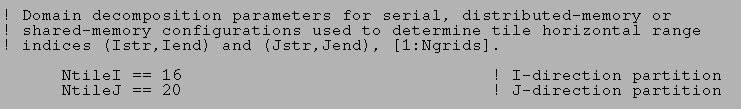
\includegraphics[width=0.80\textwidth]{roms_proc.png}
    \caption{Representation of the number of processors used in ROMS.}
    \label{romsproc}
\end{figure}
\bigskip

\subsection{WRF}
\bigskip

\noindent To change the number of WRF processors, it is necessary to modify the file \textit{namelist.input}.
You will find the variables \textit{nproc\_x} and \textit{nproc\_y}, as in Figure \textcolor{bleu_cite}{\ref{procswrf}}.
In this case, 320 processors will be reserved for the atmospheric model.

\begin{figure}[H]
    \centering
    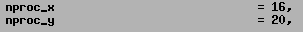
\includegraphics[width=0.50\textwidth]{wrf_proc.png}
    \caption{Representation of the number of processors for the WRF.}
    \label{procswrf}
\end{figure}
\bigskip

\subsection{SWAN}

\bigskip The SWAN \textit{.in} file does not discriminate the numbers of processors used, so just change the number
number of processors in \textit{coupling.in}, as will be shown in the subsection below.
\bigskip

\subsection{COAWST}
\bigskip

\noindent Now that the number of processors have been modified, the coupler needs to be informed about the change. 
This information is communicated through the file \textit{coupling.in}. It should contain the total number of processors 
to be used by the ROMS, WRF and SWAN models, as in the figure \textcolor{bleu_cite}{\ref{procscoa}}:
\bigskip

\begin{figure}[H]
    \centering
    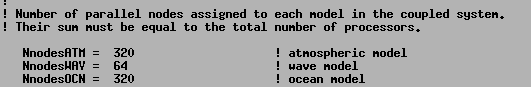
\includegraphics[width=0.80\textwidth]{taxa_acopl.png}
    \caption{Representation of the number of processors for each COAWST module.}
    \label{procscoa}
\end{figure}
\bigskip

\noindent The \textit{NnodesATM} refers to the total number of processors used by WRF, \textit{NnodesWAV} is the
total used by SWAN and \textit{NnodesOCN} is total used by ROMS. Just change according to the total number of processors used
in the previous steps.
\bigskip

\noindent Finally, it is necessary to modify the total number of processors in \textit{run.sh},used to submit the experiment.
Add the total number of processors used by the three models, following the equation \textcolor{bleu_cite}{\ref{equacao2}}:
\bigskip

\begin{equation}
TotalProc = NnodesATM + NnodesWAV + NnodesOCN
\label{equacao2}
\end{equation}
\bigskip

\noindent Where\textit{TotalProc} is the sum of all processors used in the models.
\bigskip

\noindent Now open the file \textit{run.sh}, located inside the folder \textit{Work}, and look for the following line:
\bigskip

\begin{bashcode}
\# PBS -l mppwidth= 3
\end{bashcode}
\bigskip

\noindent And for the line:
\bigskip

\begin{bashcode}
aprun -n 36 coawstM ./coupling.in 1> log.out 2> log.err
\end{bashcode}
\bigskip

\noindent Modify the number \textit{3} by the total number of processors used.
\bigskip

\section{Modifying the coupling time interval between models}
\bigskip

\noindent To modify the information exchanged between models, open the file \textit{coupling.in} and
modify the variables \textit{TI\_ATM2WAV}, \textit{TI\_ATM2OCN}, \textit{TI\_WAV2ATM}, \textit{TI\_WAV2OCN}, \textit{TI\_OCN2WAV},
          \textit{TI\_OCN2ATM}, as in Figure \textcolor{bleu_cite}{\ref{taxaacopla}}.
\bigskip

\begin{tcolorbox}[enhanced,
  grow to left by=0cm,%   equivalent to negative mdframed 'leftmargin'
  grow to right by=0cm,%  equivalent to negative mdframed 'rightmargin'
  enlarge top by=0cm,%     equivalent to mdframed 'skipabove'
  enlarge bottom by=0cm,%  equivalent to mdframed 'skipbelow'
  tcbox raise base,
  boxrule=1.0pt,
  left=18mm,
  colframe=red!50!black,coltext=red!25!black,colback=red!10!white,
  overlay={\begin{tcbclipinterior}\fill[red!75!blue!50!white] (frame.south west)
    rectangle node[text=white,font=\sffamily\bfseries\footnotesize,rotate=0] {WARNING} ([xshift=18mm]frame.north west);\end{tcbclipinterior}}]
    The information exchange rate is defined in seconds.
\end{tcolorbox}
\bigskip

\begin{figure}[H]
    \centering
    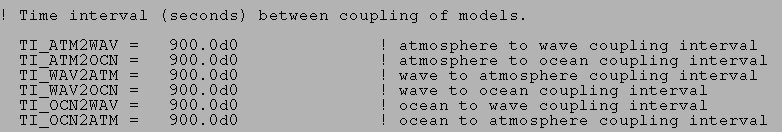
\includegraphics[width=0.95\textwidth]{coupltime.png}
    \caption{Information exchange interval between models used in COAWST. In this example, the exchange will occur every 900 seconds.}
    \label{taxaacopla}
\end{figure}
\bigskip
